\documentclass{beamer}
\usepackage[utf8]{inputenc}
\usepackage[czech]{babel}

\renewcommand{\div}{\operatorname{div}}
\newcommand{\Th}{\mathcal T_h}
\newcommand{\vc}[1]{\boldsymbol{#1}}

\begin{document}

\begin{frame}
\title{Metoda konečných prvků pro rovnici vedení tepla ve 2D}
\date{30. 11. 2016}
\maketitle
\end{frame}


\begin{frame}{Rovnice vedení tepla ve 2D}

\begin{columns}
\column{5cm}
\begin{align*}
-\Delta u + \div(u\vc q) &= 0 &&\mbox{ v }\Omega\\
u &= 1 &&\mbox{ na }\Gamma_d\\
\nabla u \cdot\vc n &= 0 &&\mbox{ na }\Gamma_n
\end{align*}

\begin{align*}
\Gamma_d &= \{ \vc x\in\partial\Omega;~\vc q(\vc x)\cdot\vc n < 0 \}\\
\Gamma_n &= \partial\Omega\setminus\Gamma_d
\end{align*}


\column{7cm}
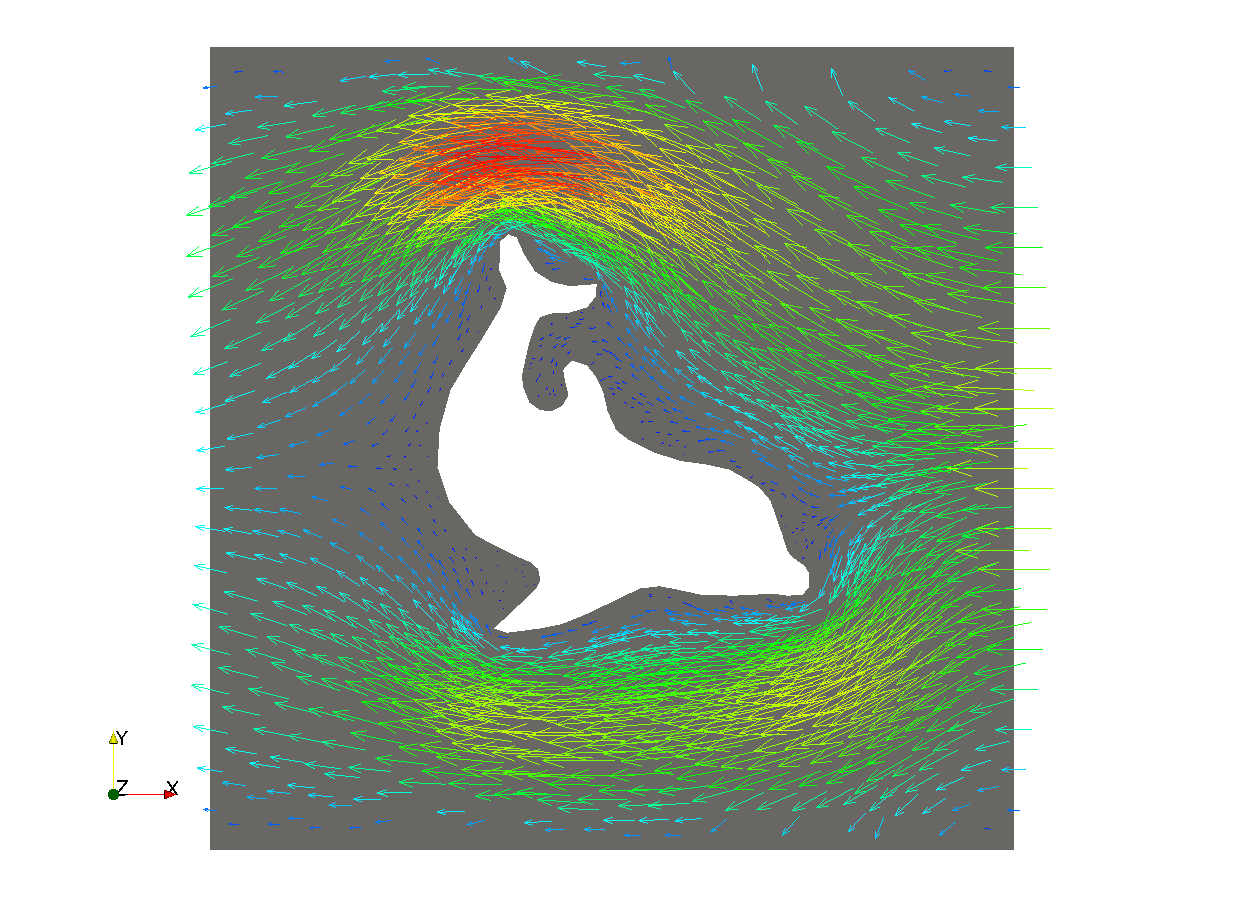
\includegraphics[width=7cm]{velocity}
\end{columns}

Slabá formulace:

Najdi $u\in H^1(\Omega)$ takové, že
\begin{itemize}
\item $z:=u-1\in V:=H^1_{\Gamma_d}(\Omega)$
\item $\forall v\in V:~\underbrace{(\nabla z,\nabla v) - (z\vc q,\nabla v)+(z\vc q\cdot\vc n,v)_{\Gamma_n}}_{a(z,v)} = \underbrace{(\vc q,\nabla v)-(\vc q\cdot\vc n,v)_{\Gamma_n}}_{l(v)}$
\end{itemize}

\end{frame}


\begin{frame}{Metoda konečných prvků}

\begin{columns}
\column{6cm}
1) Triangulace $\Th$ oblasti $\Omega$\\
$K\in \Th$...trojúhelník\\
$x_1,..., x_N$...uzlové body triangulace uvnitř oblasti
\vspace{1cm}

2) Podprostor $V_h$:

\begin{itemize}
\item spojité funkce na $\overline\Omega$
\item lineární na každém trojúhelníku $K\in \Th$
\item nulové na $\Gamma_d$
\end{itemize}
\vspace{1cm}

3) Báze $V_h$:

$\varphi_j(x_i) = \delta_{ij}$

\column{6cm}
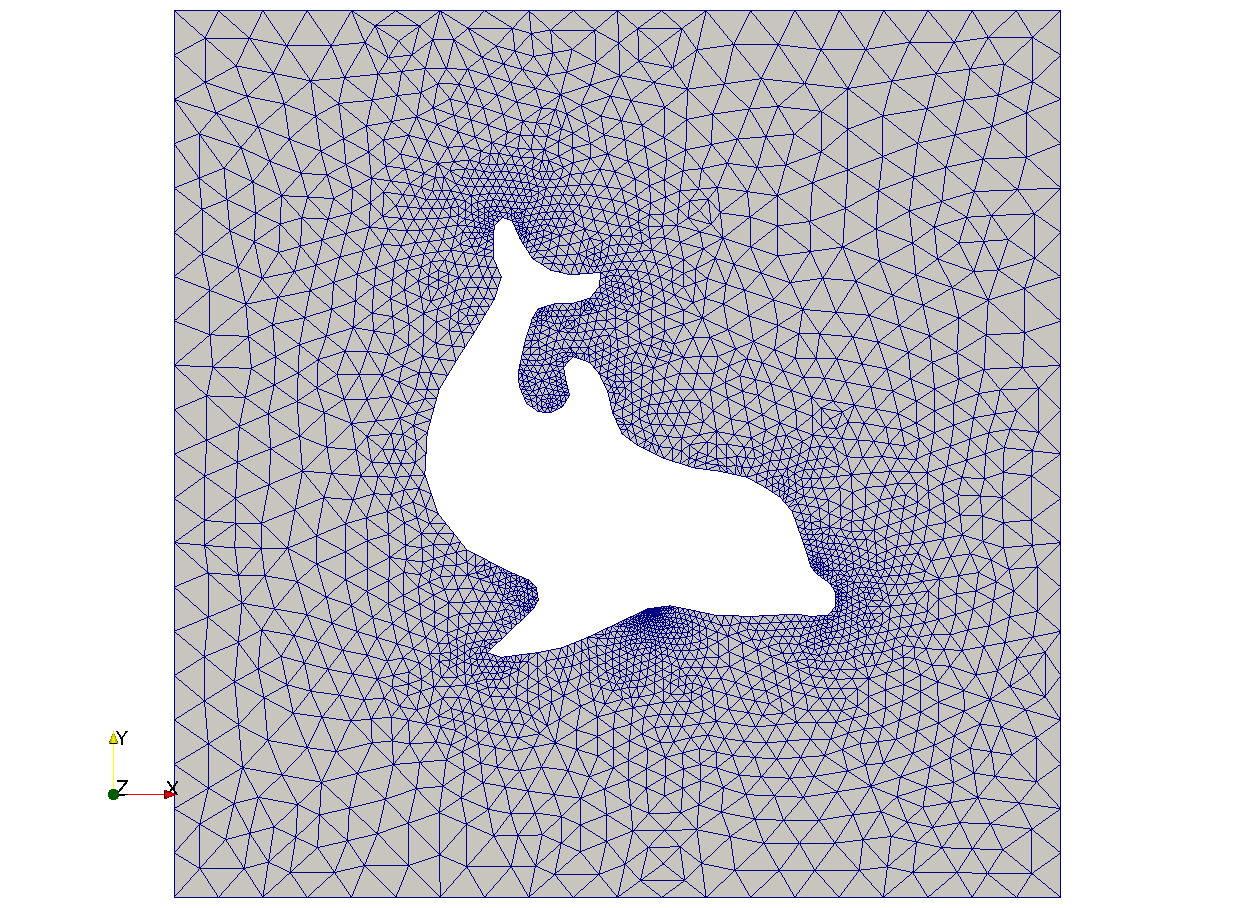
\includegraphics[width=6cm]{mesh}\\
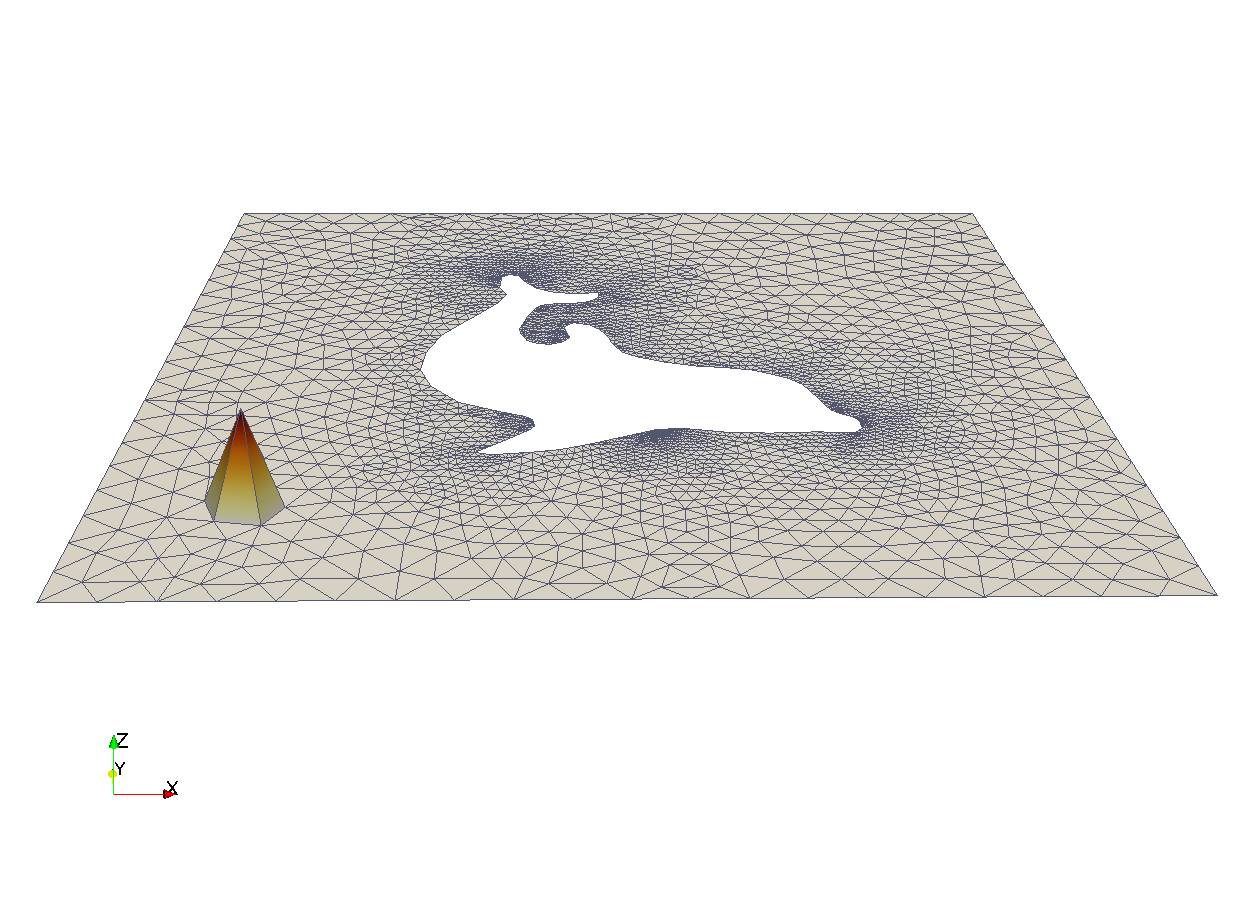
\includegraphics[width=6cm]{base}
\end{columns}

\end{frame}


\begin{frame}{Metoda konečných prvků}

4) Galerkinova aproximace:

Najdi $u_h:=1+z_h$, kde $z_h\in V_h$ řeší úlohu:
\begin{equation}\label{eq:galerkin}
\forall v_h\in V_h:~ a(z_h,v_h)=l(v_h)
\end{equation}
\bigskip

5) Algebraická soustava:\medskip

$ z_h := \sum_{i=1}^N\xi_i\varphi_i,~\vc x=(\xi_1,...,\xi_N)^\top $\medskip

$a_{ij} := a(\varphi_j,\varphi_i) = (\nabla \varphi_j,\nabla\varphi_i) - (\varphi_j\vc q,\nabla\varphi_i) + (\varphi_j\vc q\cdot\vc n,\varphi_i)_{\Gamma_n}$\medskip

$b_i := l(\varphi_i) = (\vc q,\nabla\varphi_i) - (\vc q\cdot\vc n,\varphi_i)_{\Gamma_n}$

\[ \eqref{eq:galerkin} \Leftrightarrow \mathbb A\vc x = \vc b\]

Výpočet integrálů v $a_{ij}$: $(\nabla\varphi_j,\nabla\varphi_i)=\sum_{K\in\Th}\int_K\nabla\varphi_j\cdot\nabla\varphi_i$ - sčítá se pouze přes elementy $K$, na kterých je $\varphi_i$ i $\varphi_j$ nenulové.

\end{frame}


\begin{frame}{Numerické řešení $u_h$}

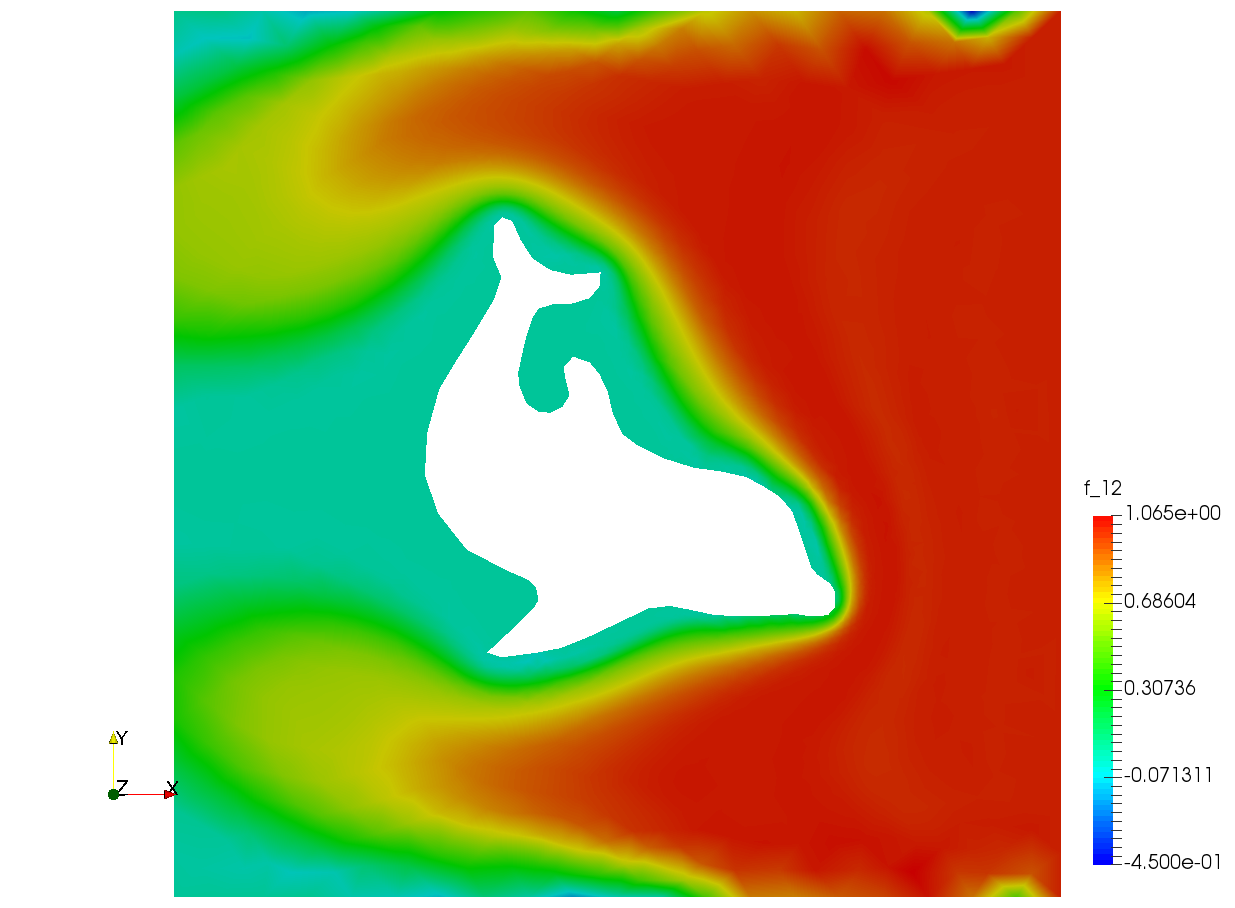
\includegraphics[width=6cm]{temp}
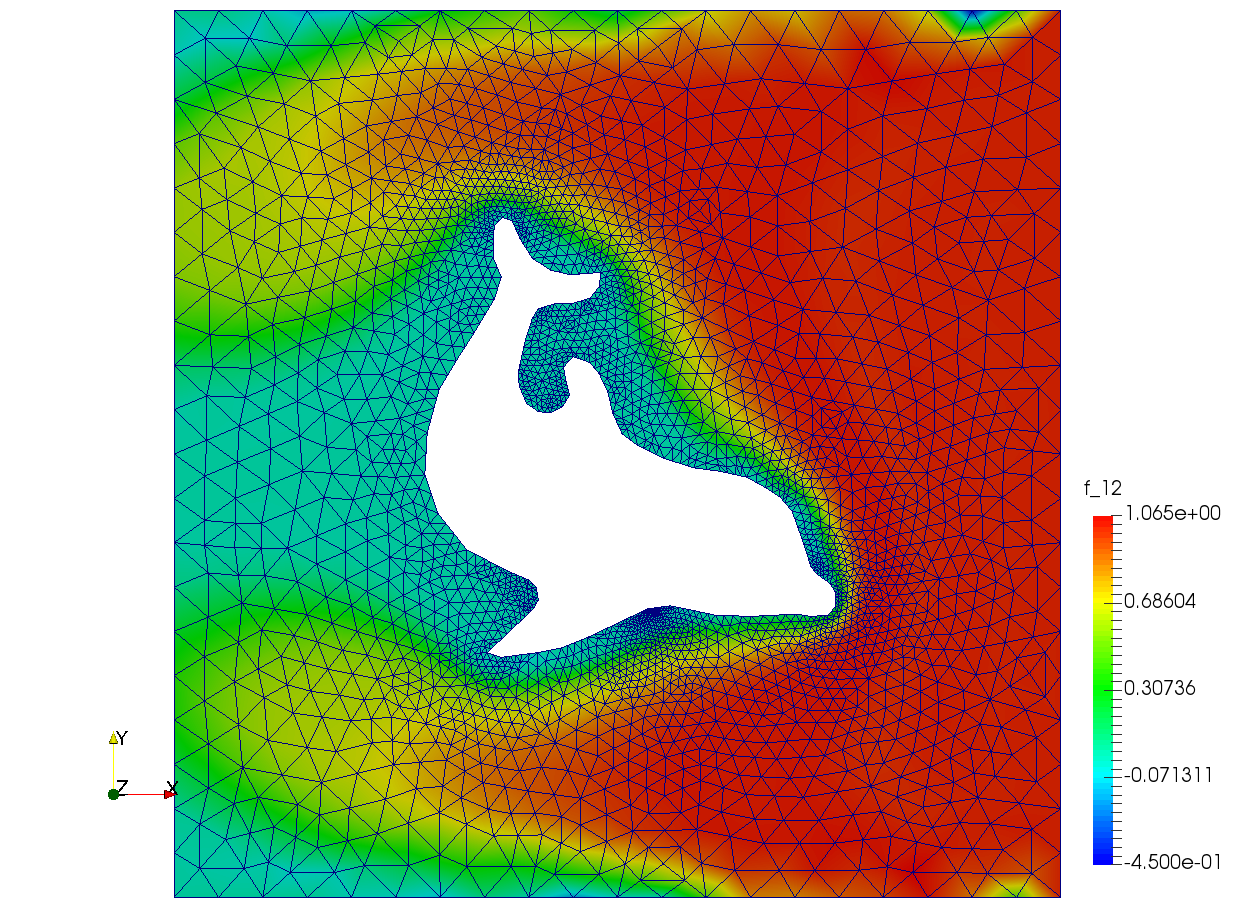
\includegraphics[width=6cm]{temp_mesh}

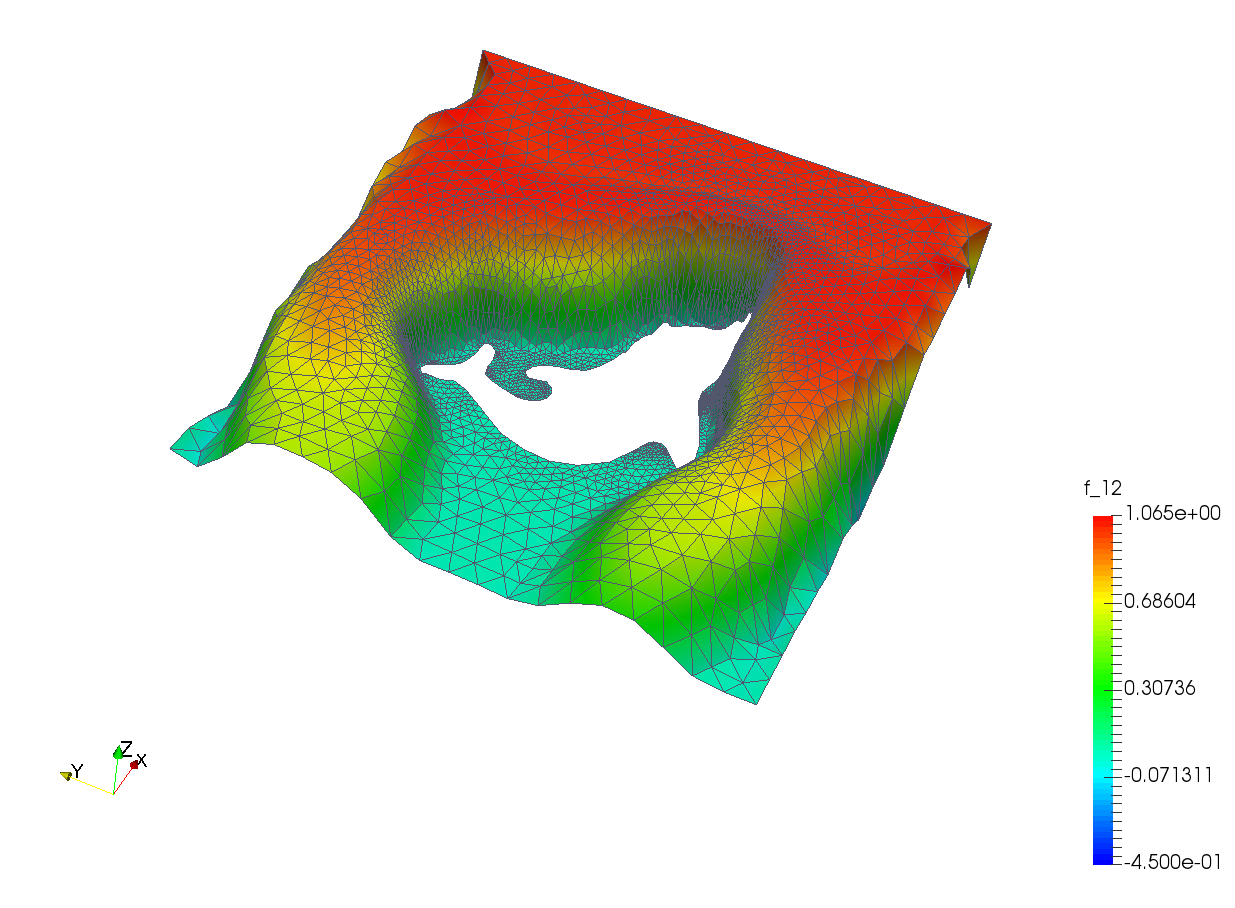
\includegraphics[width=6cm]{temp_3d}

\end{frame}

\end{document}